\documentclass[letterpaper,11pt,oneside]{book}
\usepackage[lmargin=2.5cm,
rmargin=2.5cm,top=2.7cm,bottom=3.3cm]{geometry}

\usepackage[utf8]{inputenc}
\usepackage[spanish]{babel} 

\usepackage{tikz,lipsum,lmodern}
\usepackage[most]{tcolorbox}

\usepackage{cancel}


\usepackage{amsmath}
\usepackage{graphicx}
\usepackage{graphics}
\usepackage{enumitem}
\usepackage{pdfpages}

\usepackage{pgf,tikz,pgfplots}
\pgfplotsset{compat=1.15}
\usepackage{mathrsfs}
\usetikzlibrary{arrows}
%\usepackage{fontspec}

\usepackage{xcolor}
\usepackage{gensymb}
\usepackage{hyperref}
\usepackage{float}
\usepackage{tikz}
%\usepackage[spanish,es-noshorthands]{babel}
\usepackage{xcolor}
\usepackage{amsthm}
\usepackage{amsfonts}
%\usepackage[shortlabels]{enumitem}
\usepackage{multicol}
%\usepackage{pdfpages}
%\usepackage[centering,text ={18 cm ,22 cm } , showframe = false]{geometry}

\usepackage{xparse} % paquete para hacer entornos con p a r m e t r o s

\newtheoremstyle{break}
{\topsep}{\topsep}%
{\itshape}{}%
{\bfseries}{}%
{\newline}{}%

\theoremstyle{definition}
\newtheorem{exer}{$\textit{\textbf{Ejercicio}}$}[section]
\newtheorem{exers}{Ejercicios}[section]
\newtheorem{ejemplo}{{ Ejemplo }}[section]

%\theoremstyle{theorem}
\newtheorem{theorem}{{ Teorema }}[chapter]
\newtheorem{prop}{{ Propiedad }}[chapter]
\newtheorem{defi}{{\underline{\textbf Definici\'on}}}[chapter]
\newtheorem{problem}{\textbf{\textit Problema}}[chapter]
\theoremstyle{remark}
\newtheorem{act}{ \textbf{Actividad} }[section]
\newtheorem{act_clase}{ \textbf{Actividad de Clase} }[section]


\begin{document}
	
	\begin{titlepage}
		\begin{center}
			\begin{Huge}
				\textsc{Recopilación de pruebas}
			\end{Huge}
		\end{center}
	\end{titlepage}
	
	\newpage
	$\ $
	\thispagestyle{empty} % para que no se numere esta pagina
	
	\chapter*{}
	\pagenumbering{Roman} % para comenzar la numeracion de paginas en numeros romanos
	\begin{flushright}
		\textit{Dedicado a todos aquellos que ven mas all\'a de los n\'umeros}
	\end{flushright}
	
	\newpage
	$\ $
	\thispagestyle{empty}
	
	
	\tableofcontents
	
	\newpage
	$\ $
	\thispagestyle{empty} % para que no se numere esta pagina
	
	\pagenumbering{arabic} % para empezar la numeraci�n con n�meros	
	
	\chapter{23 de Mayo de 2020}\label{chap:23mayo2020}
	\newpage
\section*{Referencias}
\textbf{Básico: } Prueba de la ronda Final de OMAPA 2012, Nivel 1, Grados 6 y 7. \\
\textbf{Medio: } Prueba de la ronda Final de OMAPA 2012, Nivel 2, Grados 8 y 9. \\
\textbf{Avanzado: } Prueba de la ronda Final de OMAPA 2012, Nivel 3, Grados 10 y 11

%------------------------------------------------------------------------------------------------------------   
%----------------------------------                        BASICO                       ---------------------------------- 
%------------------------------------------------------------------------------------------------------------ 

\newpage
\section{Nivel Básico}\label{BASICO_2020_23_mayo}

\begin{center}
	\fbox{\fbox{\parbox{6in}{\centering
				\textbf{Tiempo mínimo: } 2 horas y 30 minutos.\\
				\textbf{Tiempo máximo: } 4 horas.\\	
				\textbf{Procedimientos: }Cada problema debe estar resuelto por escrito, en forma detallada, todos los pasos seguidos para su resolución deben estar bien explicados. Se le brindarán unas hojas grapadas, en la \textit{parte de enfrente} de cada hoja debe estar la solución de los problemas, la \textit{parte posterior} no se leerá pero las operaciones y cálculos deben hacerlos allí. \\
				\textbf{Puntaje: }Cada problema vale 50 puntos, son 5, para un total de 250 puntos.
				}}}
\end{center}


\begin{figure}[H]
	\centering
	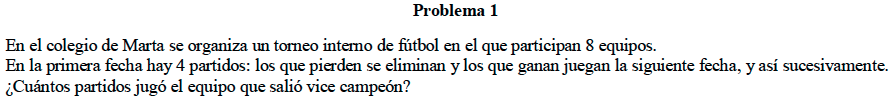
\includegraphics[width=\linewidth]{2020_05_23/imgs/OMAPA_2012_r5_B_1}
	%\caption{}
	\label{OMAPA_2012_r5_B_1}
\end{figure}

\begin{figure}[H]
	\centering
	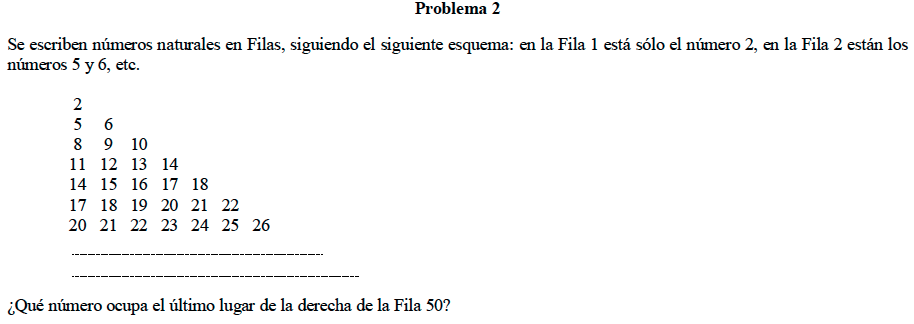
\includegraphics[width=\linewidth]{2020_05_23/imgs/OMAPA_2012_r5_B_2}
	%\caption{}
	\label{OMAPA_2012_r5_B_2}
\end{figure}

\begin{figure}[H]
	\centering
	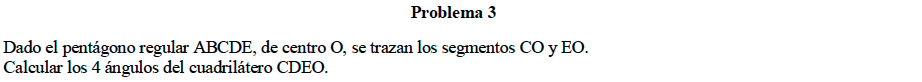
\includegraphics[width=\linewidth]{2020_05_23/imgs/OMAPA_2012_r5_B_3}
	%\caption{}
	\label{OMAPA_2012_r5_B_3}
\end{figure}

\begin{figure}[H]
	\centering
	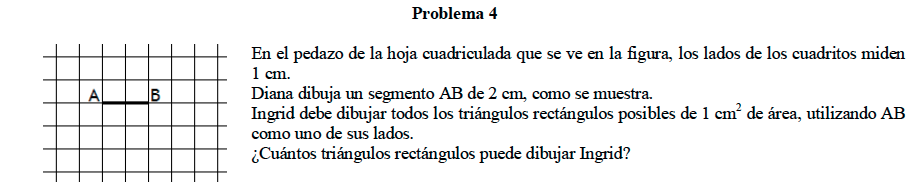
\includegraphics[width=\linewidth]{2020_05_23/imgs/OMAPA_2012_r5_B_4}
	%\caption{}
	\label{OMAPA_2012_r5_B_4}
\end{figure}

\begin{figure}[H]
	\centering
	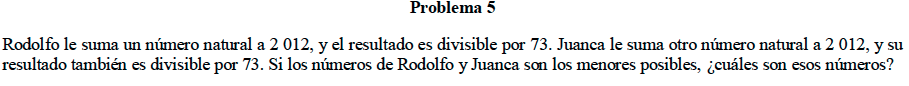
\includegraphics[width=\linewidth]{2020_05_23/imgs/OMAPA_2012_r5_B_5}
	%\caption{}
	\label{OMAPA_2012_r5_B_5}
\end{figure}

%------------------------------------------------------------------------------------------------------------   
%----------------------------------                        MEDIO                       ---------------------------------- 
%------------------------------------------------------------------------------------------------------------ 
\newpage
\section{Nivel Medio}\label{MEDIO_2020_23_mayo}

\begin{center}
	\fbox{\fbox{\parbox{6in}{\centering
				\textbf{Tiempo mínimo: } 2 horas y 30 minutos.\\
				\textbf{Tiempo máximo: } 4 horas.\\				
				\textbf{Procedimientos: }Cada problema debe estar resuelto por escrito, en forma detallada, todos los pasos seguidos para su resolución deben estar bien explicados. Se le brindarán unas hojas grapadas, en la \textit{parte de enfrente} de cada hoja debe estar la solución de los problemas, la \textit{parte posterior} no se leerá pero las operaciones y cálculos deben hacerlos allí. \\
				\textbf{Puntaje: }Cada problema vale 50 puntos, son 5, para un total de 250 puntos.
	}}}
\end{center}


\begin{figure}[H]
	\centering
	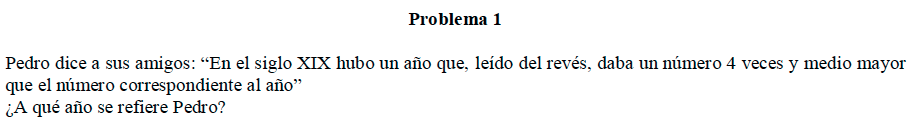
\includegraphics[width=\linewidth]{2020_05_23/imgs/OMAPA_2012_r5_M_1}
	%\caption{}
	\label{OMAPA_2012_r5_M_1}
\end{figure}

\begin{figure}[H]
	\centering
	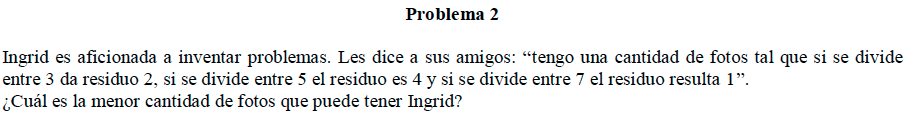
\includegraphics[width=\linewidth]{2020_05_23/imgs/OMAPA_2012_r5_M_2}
	%\caption{}
	\label{OMAPA_2012_r5_M_2}
\end{figure}

\begin{figure}[H]
	\centering
	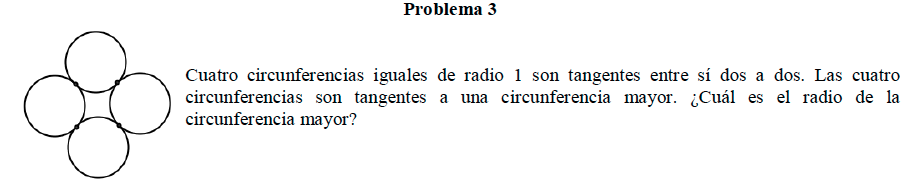
\includegraphics[width=\linewidth]{2020_05_23/imgs/OMAPA_2012_r5_M_3}
	%\caption{}
	\label{OMAPA_2012_r5_M_3}
\end{figure}

\begin{figure}[H]
	\centering
	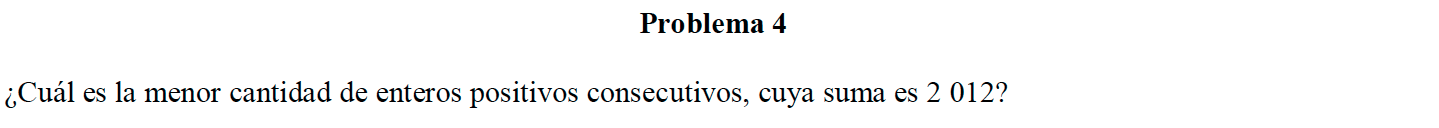
\includegraphics[width=\linewidth]{2020_05_23/imgs/OMAPA_2012_r5_M_4}
	%\caption{}
	\label{OMAPA_2012_r5_M_4}
\end{figure}

\begin{figure}[H]
	\centering
	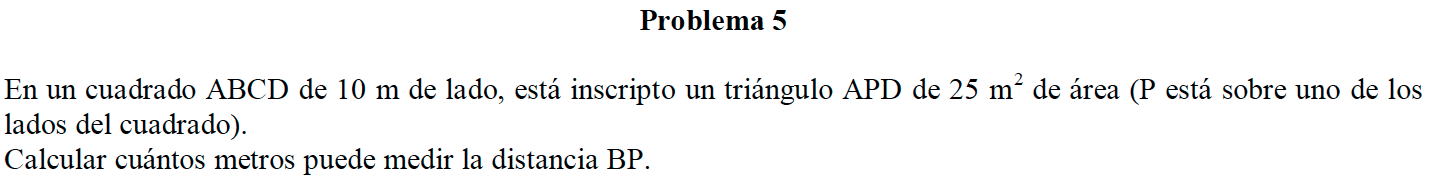
\includegraphics[width=\linewidth]{2020_05_23/imgs/OMAPA_2012_r5_M_5}
	%\caption{}
	\label{OMAPA_2012_r5_M_5}
\end{figure}

%------------------------------------------------------------------------------------------------------------   
%----------------------------------                        AVANZADO                       ---------------------------------- 
%------------------------------------------------------------------------------------------------------------ 

\newpage
\section{Nivel Avanzado}\label{AVANZADO_2020_23_mayo}

\begin{center}
	\fbox{\fbox{\parbox{6in}{\centering
				\textbf{Tiempo mínimo: } 2 horas y 30 minutos.\\
				\textbf{Tiempo máximo: } 4 horas.\\		
				\textbf{Procedimientos: }Cada problema debe estar resuelto por escrito, en forma detallada, todos los pasos seguidos para su resolución deben estar bien explicados. Se le brindarán unas hojas grapadas, en la \textit{parte de enfrente} de cada hoja debe estar la solución de los problemas, la \textit{parte posterior} no se leerá pero las operaciones y cálculos deben hacerlos allí. \\
				\textbf{Puntaje: }Cada problema vale 50 puntos, son 5, para un total de 250 puntos.
	}}}
\end{center}


\begin{figure}[H]
	\centering
	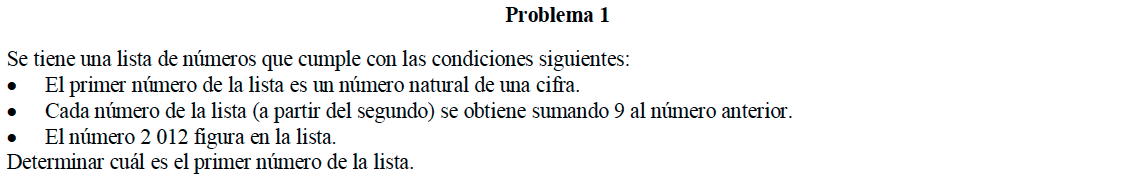
\includegraphics[width=\linewidth]{2020_05_23/imgs/OMAPA_2012_r5_A_1}
	%\caption{}
	\label{OMAPA_2012_r5_A_1}
\end{figure}

\begin{figure}[H]
	\centering
	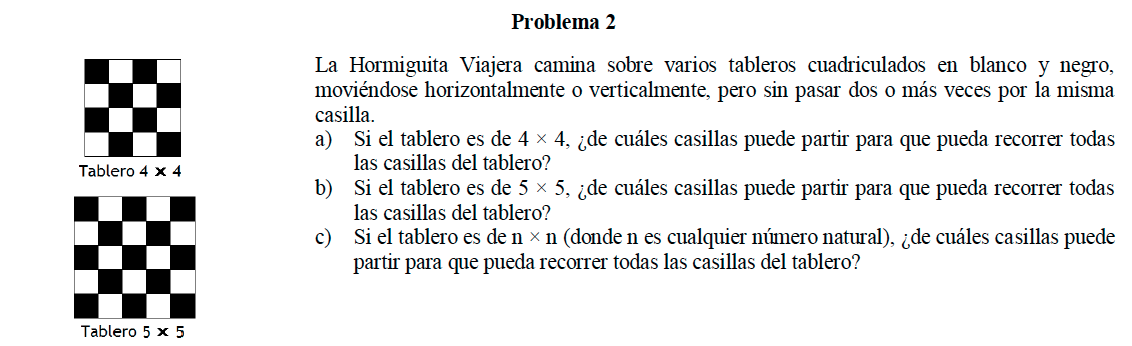
\includegraphics[width=\linewidth]{2020_05_23/imgs/OMAPA_2012_r5_A_2}
	%\caption{}
	\label{OMAPA_2012_r5_A_2}
\end{figure}

\begin{figure}[H]
	\centering
	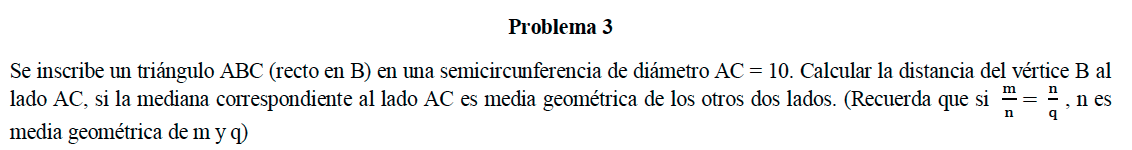
\includegraphics[width=\linewidth]{2020_05_23/imgs/OMAPA_2012_r5_A_3}
	%\caption{}
	\label{OMAPA_2012_r5_A_3}
\end{figure}

\begin{figure}[H]
	\centering
	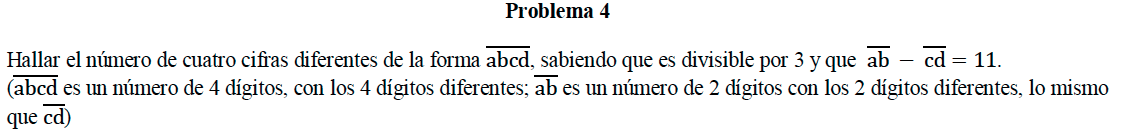
\includegraphics[width=\linewidth]{2020_05_23/imgs/OMAPA_2012_r5_A_4}
	%\caption{}
	\label{OMAPA_2012_r5_A_4}
\end{figure}

\begin{figure}[H]
	\centering
	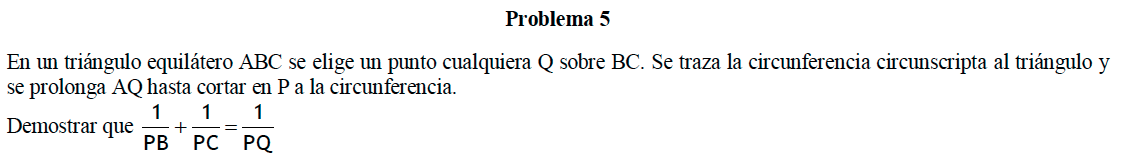
\includegraphics[width=\linewidth]{2020_05_23/imgs/OMAPA_2012_r5_A_5}
	%\caption{}
	\label{OMAPA_2012_r5_A_5}
\end{figure}
	
	\chapter{13 de Junio de 2020}\label{chap:13junio2020}
	\newpage

\section*{Referencias}
\textbf{Básico: }
		\begin{itemize}
			\item \textit{Problema 1} tomado de OPM 2017-2018 Pre-olimpiadas 5ano problema 2. 
			\item \textit{Problema 2} tomado de OPM 2017-2018 Pre-olimpiadas 5ano problema 3.
			\item \textit{Problema 3} tomado de OPM 2017-2018 $2\degree$ eliminatoria, Junior problema 1.
			\item \textit{Problema 4} tomado de OPM 2017-2018 $2\degree$ eliminatoria, Junior problema 3.
		\end{itemize}
	
\textbf{Medio: }
\begin{itemize}
	\item \textit{Problema 1} tomado de OPM 2017-2018 $2\degree$ eliminatoria, Junior problema 3.
	\item \textit{Problema 2} tomado de OPM 2017-2018 $2\degree$ eliminatoria, Junior problema 4.
	\item \textit{Problema 3} tomado de OPM 2017-2018 $2\degree$ eliminatoria, Categoria A problema 1.
	\item \textit{Problema 4} tomado de OPM 2017-2018 $2\degree$ eliminatoria, Categoria A problema 4.
\end{itemize}

\textbf{Avanzado: }
\begin{itemize}
	\item \textit{Problema 1} tomado de OPM 2017-2018 $2\degree$ eliminatoria, Categoria A problema 3.
	\item	\textit{Problema 2} tomado de OPM 2017-2018 $2\degree$ eliminatoria, Categoria B problema 1.
	\item	\textit{Problema 4} tomado de OPM 2017-2018 $2\degree$ eliminatoria, Categoria B problema 2.
	\item	\textit{Problema 5} tomado de OPM 2016-2017 Final día 1, Categoria B problema 1.
\end{itemize}



%------------------------------------------------------------------------------------------------------------   
%----------------------------------                        BASICO                       ---------------------------------- 
%------------------------------------------------------------------------------------------------------------ 
\newpage
\section{Nivel Básico}\label{BASICO_2020_13_junio}
\begin{center}
	\fbox{\fbox{\parbox{6in}{\centering
				\textbf{Tiempo mínimo: } 2 horas y 30 minutos.\\
				\textbf{Tiempo máximo: } 4 horas.\\	
				\textbf{Procedimientos: }Cada problema debe estar resuelto por escrito, en forma detallada, todos los pasos seguidos para su resolución deben estar bien explicados. Se le brindarán unas hojas grapadas, en la \textit{parte de enfrente} de cada hoja debe estar la solución de los problemas, la \textit{parte posterior} no se leerá pero la pueden usar como borrador de los problemas\\
				\textbf{Puntaje máximo: }250 puntos.
	}}}
\end{center}

\begin{enumerate}
\item \textbf{50 puntos}. José tenía un terreno rectangular del cuál vendió una parte rectangular mas pequeña, quedandose solamente con un terreno de área $68m^2$, las medidas se muestran en la figura. El señor José pretende comprar una red para cercar su terreno. Sabiendo que el metro de red cuesta $50$ pesos, cuánto tendrá que gastar José para cercar su terreno?
		\begin{figure}[H]
			\centering
			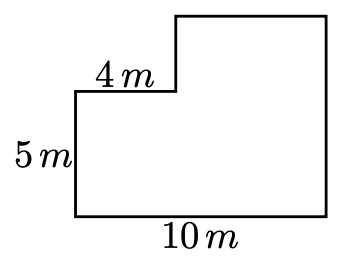
\includegraphics[width=0.4\linewidth]{2020_06_13/imgs/basic_p1}
			%\caption{}
			\label{basicp1}
		\end{figure}

\item \textbf{50 puntos}. Andrés tiene un trompo y quiere pintar los tres triángulos que tiene en su forma usando los colores amarillo, azul y rojo. Si Andrés quiere poder pintar regiones diferentes del mismo color, de cuántas maneras en total puede pintar su trompo?
		\begin{figure}[H]
			\centering
			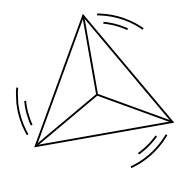
\includegraphics[width=0.2\linewidth]{2020_06_13/imgs/basic_p2}
			%\caption{}
			\label{basicp2}
		\end{figure}


\item \hspace{1cm}
	\begin{enumerate}[label=\Alph*)]
	\item \textbf{25 puntos}. Paulo es dueño de un terreno que está compuesto de tres cuadrados y tres trapecios. El área de cada cuadrado se muestra en la figura. Cuánto vale el lote sombreado sabiendo que cada $m^2$ vale 1 millón de pesos?
			\begin{figure}[H]
				\centering
				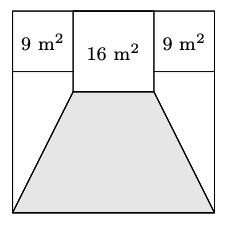
\includegraphics[width=0.4\linewidth]{2020_06_13/imgs/basic_p3_a}
				%\caption{}
				\label{basicp3a}
			\end{figure}
		
	\item \textbf{25 puntos}. Considere la siguiente lista de afirmaciones:
			\begin{enumerate}
			\item En esta lista hay exactamente una afirmación falsa.
			\item En esta lista hay exactamente dos afirmaciones falsas.
			\item En esta lista hay exactamente tres afirmaciones falsas.
			\item En esta lista hay exactamente cuatro afirmaciones falsas.			
			\end{enumerate}
			Cuál de las afirmaciones es verdadera? o ninguna es verdadera? 
			
	\item \textbf{25 puntos}. En cuántos ceros termina el número $8^7\times 25^5$?
	
	\item \textbf{25 puntos}. Un número de tres dígitos se dice que es \textit{cuadriñado} si es multiplo de cuatro y todos los números que se obtienen al desordenar sus dígitos también son múltiplos de cuatro. Por ejemplo, 408 es \textit{cuadriñado} porque 408, 084, 048, 840 y 804 son todos múltiplos de cuatro. Cuántos números \textit{cuadriñados existen}?
	\end{enumerate}

\item \textbf{50 puntos}. En un triángulo $CDE$, el punto $A$ está en $CD$ de forma que la distancia de $A$ a $C$ es $4cm$ y de $A$ a $D$ $8cm$. El punto $B$ está en $CE$ a $6cm$ de $C$ y $2cm$ de $E$. Si el área del triángulo $ABC$ es $3{cm}^2$, cuánto mide el área del triángulo $CDE$?


\end{enumerate}

%------------------------------------------------------------------------------------------------------------   
%----------------------------------                        MEDIO                       ---------------------------------- 
%------------------------------------------------------------------------------------------------------------ 

\newpage
\section{Nivel Medio}\label{MEDIO_2020_13_junio}

\begin{center}
	\fbox{\fbox{\parbox{6in}{\centering
				\textbf{Tiempo mínimo: } 2 horas y 30 minutos.\\
				\textbf{Tiempo máximo: } 4 horas.\\	
				\textbf{Procedimientos: }Cada problema debe estar resuelto por escrito, en forma detallada, todos los pasos seguidos para su resolución deben estar bien explicados. Se le brindarán unas hojas grapadas, en la \textit{parte de enfrente} de cada hoja debe estar la solución de los problemas, la \textit{parte posterior} no se leerá pero la pueden usar como borrador de los problemas\\
				\textbf{Puntaje máximo: }250 puntos.
	}}}
\end{center}

\begin{enumerate}
\item \textbf{50 puntos}. En un triángulo $CDE$, el punto $A$ está en $CD$ de forma que la distancia de $A$ a $C$ es $4cm$ y de $A$ a $D$ $8cm$. El punto $B$ está en $CE$ a $6cm$ de $C$ y $2cm$ de $E$. Si el área del triángulo $ABC$ es $3{cm}^2$, cuánto mide el área del triángulo $CDE$?

\item \textbf{50 puntos}. Siete amigos se sientan en una mesa a comer. De cuántas formas podemos escoger un grupo, por con lo menos una persona, de forma que no hayan dos personas que hayan estado sentadas al lado en la comida?

\item \hspace{1cm}
		\begin{enumerate}[label=\Alph*)]
			\item \textbf{25 puntos}. Paulo es dueño de un terreno que está compuesto de siete divisiones rectangulares como muestra la figura. El área algunas divisiones se muestra en la figura. Cuánto es el área del terreno de Paulo?
			\begin{figure}[H]
				\centering
				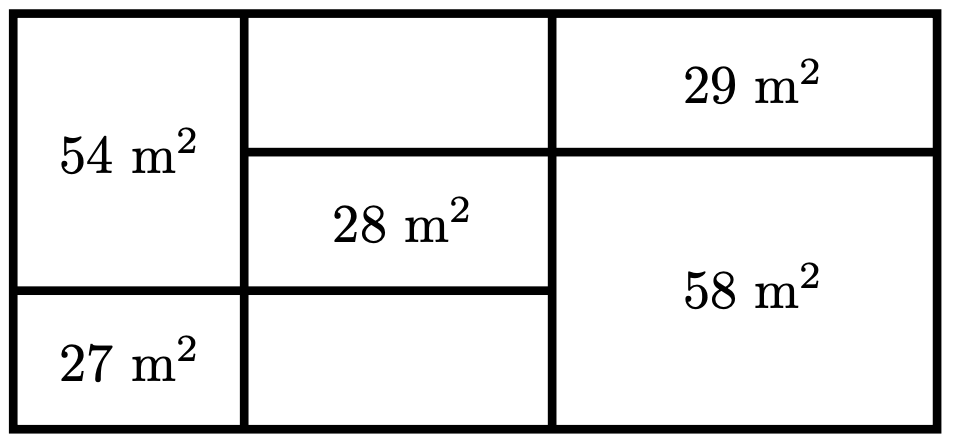
\includegraphics[width=0.4\linewidth]{2020_06_13/imgs/medio_p3_a}
				%\caption{}
				\label{medio_p3_a}
			\end{figure}
			
			\item \textbf{25 puntos}. En cuántos ceros termina el número $8^7\times 25^5$?
			
			\item \textbf{25 puntos}.  Juan nació entre 1989 y 1999 y solo sabe que una de las siguientes afirmaciones es falsa: ``Juan nació en un año par", ``Juan nació en un año múltiplo de 5", ``Juan nació en un año divisible por 3". Cuánto es el número de intentos necesarios para saber con certeza el año de nacimiento de Juan?
			
			\item \textbf{25 puntos}. Un número de tres dígitos se dice que es \textit{cuadriñado} si es multiplo de cuatro y todos los números que se obtienen al desordenar sus dígitos también son múltiplos de cuatro. Por ejemplo, 408 es \textit{cuadriñado} porque 408, 084, 048, 840 y 804 son todos múltiplos de cuatro. Cuántos números \textit{cuadriñados existen}?
		\end{enumerate}

\item \textbf{50 puntos}. En un juego de dardos, un jugador puede obtener 7 o 11 puntos en cada lanzamiento. La puntuacion de cada jugador es la suma de los puntos obtenidos en sus lanzamientos. Cuántos múltiplos de 5 son imposibles de obtener como puntuación en este juego, si no hay un límite de número de lanzamientos?
\end{enumerate}

%------------------------------------------------------------------------------------------------------------   
%----------------------------------                        AVANZADO                       ---------------------------------- 
%------------------------------------------------------------------------------------------------------------ 
\newpage
\section{Nivel Avanzado}\label{AVANZADO_2020_13_junio}

\begin{center}
	\fbox{\fbox{\parbox{6in}{\centering
				\textbf{Tiempo mínimo: } 2 horas y 30 minutos.\\
				\textbf{Tiempo máximo: } 4 horas.\\	
				\textbf{Procedimientos: }Cada problema debe estar resuelto por escrito, en forma detallada, todos los pasos seguidos para su resolución deben estar bien explicados. Se le brindarán unas hojas grapadas, en la \textit{parte de enfrente} de cada hoja debe estar la solución de los problemas, la \textit{parte posterior} no se leerá pero la pueden usar como borrador de los problemas\\
				\textbf{Puntaje máximo: }250 puntos.
	}}}
\end{center}

\begin{enumerate}
	\item \textbf{50 puntos}. Para desbloquear su celular, Juan utiliza contraseñas de 4 dígitos diferentes de cero de forma que el primer dígito es la suma de los otros tres. Si Juan cambia la contraseña todos los días, luego de cuántos días Juan se verá obligado a repetir contraseña?
	
	\item \textbf{50 puntos}. Cuál es el mayor múltiplo de 3 que no puede ser escrito de la forma $7a+11b$, donde $a$ y $b$ son números naturales?
	
	\item \textbf{50 puntos}. Diez amigos se sientan en una mesa a comer. De cuántas formas podemos escoger un grupo, por con lo menos una persona, de forma que no hayan dos personas que hayan estado sentadas al lado en la comida?
	
	\item \textbf{50 puntos}. Sea $\triangle ABC$ de área 9 y $D,E$ y $F$ puntos en los lados $AB, BC$ y $AC$ respectivamente tales que $DE\parallel AC$ y $DF\parallel BC$. Sabiendo que el área de $\triangle DEB$ es cuatro veces el área de $\triangle AFD$, cuál es el área de $\triangle CFE$?	
			\begin{figure}[H]
				\centering
				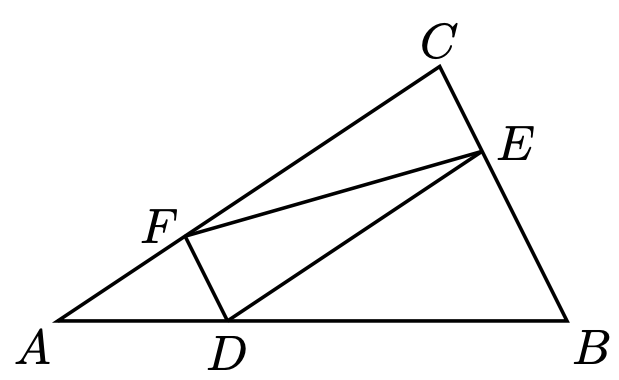
\includegraphics[width=0.45\linewidth]{2020_06_13/imgs/AV_P4}
				%\caption{}
				\label{avp4}
			\end{figure}
		
	\item \textbf{50 puntos}. Determinar todos los valores \textbf{enteros} de $n$ para los cuales el número
	\[\frac{14n+25}{2n+1}\]
	es un cuadrado perfecto.
	
\end{enumerate}

	\chapter{15 de Agosto de 2020}\label{chap:15agosto2020}
	\newpage
\section*{Referencias}
\textbf{Básico: }
\begin{itemize}
	\item \textit{Problema 1.} Problema 1 Final UIS 2018 Nivel Avanzado Primaria. 
	\item \textit{Problema 2.} Problema 2 Final UIS 2018 Nivel Avanzado Primaria. 
	\item \textit{Problema 3.} Problema 8 Selectiva UIS 2012 Nivel Medio Primaria.
	\item \textit{Problema 4.} Problema 9 Selectiva UIS 2012 Nivel Medio Primaria.
	\item \textit{Problema 5.} Creado.
\end{itemize}

\textbf{Avanzado: }
\begin{itemize}
	\item \textit{Problema 1.} Problema 8 Selectiva UIS 2019 Nivel Avanzado
	\item	\textit{Problema 2.} Problema 2 Selectiva UIS 2018 Nivel Avanzado
	\item	\textit{Problema 3.} 4.55 de \textit{Introduction to Number Thoery (AOPS)}
	\item	\textit{Problema 4.} Problema 2 Geometría N.2 A.4 de POTI (	Programa Olímpico de Treinamento)
	\item	\textit{Problema 5.} 2.31 de David Patrick. \textit{Introduction to Counting and Probability}. Aops, 2005.
\end{itemize}

%------------------------------------------------------------------------------------------------------------   
%----------------------------------                        BASICO                       ---------------------------------- 
%------------------------------------------------------------------------------------------------------------ 

\newpage
\section{Nivel Básico}\label{basico:2020_15_agosto}

\begin{center}
	\fbox{\fbox{\parbox{6in}{\centering
				\textbf{Tiempo mínimo: } 2 horas y 30 minutos.\\
				\textbf{Tiempo máximo: } 4 horas.\\	
				\textbf{Procedimientos: }Cada problema debe estar resuelto por escrito, en forma detallada, todos los pasos seguidos para su resolución deben estar bien explicados. Se le brindarán unas hojas grapadas, en la \textit{parte de enfrente} de cada hoja debe estar la solución de los problemas, la \textit{parte posterior} no se leerá pero las operaciones y cálculos deben hacerlos allí. \\
				\textbf{Puntaje: }Cada problema vale 50 puntos, son 5, para un total de 250 puntos.
				}}}
\end{center}

\begin{enumerate}
	\item \textbf{(50 puntos)}. 
				\begin{figure}[H]
					\centering
					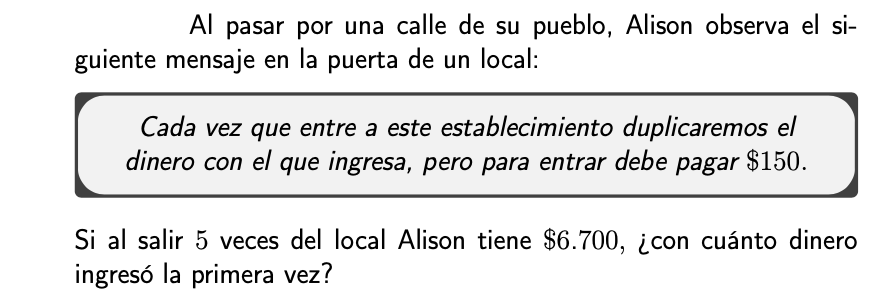
\includegraphics[width=0.95\linewidth]{2020_08_15/imgs/basicoproblema1}
					%\caption{}
					\label{fig:basicoproblema1}
				\end{figure}
			
	\item \textbf{(50 puntos)}. 
				\begin{figure}[H]
					\centering
					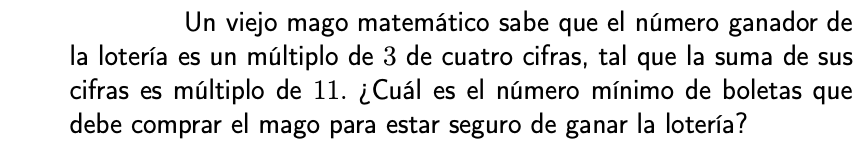
\includegraphics[width=0.95\linewidth]{2020_08_15/imgs/basicoproblema2}
					%\caption{}
					\label{fig:basicoproblema2}
				\end{figure}
	
		\item \textbf{(50 puntos)}. 
				\begin{figure}[H]
					\centering
					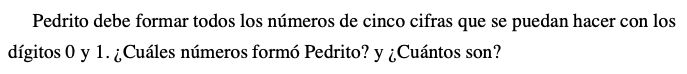
\includegraphics[width=0.95\linewidth]{2020_08_15/imgs/p8basico}
					%\caption{}
					\label{fig:basicoproblema3}
				\end{figure}

	\item \textbf{(50 puntos)}. 
			\begin{figure}[H]
				\centering
				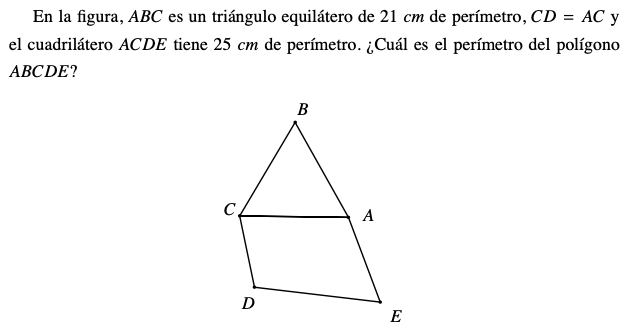
\includegraphics[width=0.95\linewidth]{2020_08_15/imgs/p9basico}
				%\caption{}
				\label{fig:basicoproblema4}
			\end{figure}
		
	\item \textbf{(50 puntos)}. Calcular el resultado de la siguiente operación:
	\[
	\frac{100-101+102-103+104-105+106-\cdots +198-199+200}{50}
	\]
\end{enumerate}



%------------------------------------------------------------------------------------------------------------   
%----------------------------------                        AVANZADO                       ---------------------------------- 
%------------------------------------------------------------------------------------------------------------ 

\newpage
\section{Nivel Avanzado}\label{avanzado:2020_15_agosto}

\begin{center}
	\fbox{\fbox{\parbox{6in}{\centering
				\textbf{Tiempo mínimo: } 2 horas y 30 minutos.\\
				\textbf{Tiempo máximo: } 4 horas.\\		
				\textbf{Procedimientos: }Cada problema debe estar resuelto por escrito, en forma detallada, todos los pasos seguidos para su resolución deben estar bien explicados. Se le brindarán unas hojas grapadas, en la \textit{parte de enfrente} de cada hoja debe estar la solución de los problemas, la \textit{parte posterior} no se leerá pero las operaciones y cálculos deben hacerlos allí. \\
				\textbf{Puntaje: }Cada problema vale 50 puntos, son 5, para un total de 250 puntos.
	}}}
\end{center}


\begin{enumerate}
		\item \textbf{(50 puntos)}. 
		\begin{figure}[H]
			\centering
			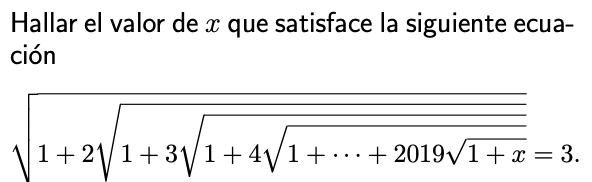
\includegraphics[width=0.6\linewidth]{2020_08_15/imgs/p8selectivavanzado2019}
			%\caption{}
			\label{fig:p8selectivavanzado2019}
		\end{figure}

\item \textbf{(50 puntos)}. 
		\begin{figure}[H]
			\centering
			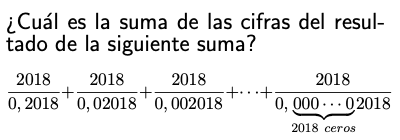
\includegraphics[width=0.6\linewidth]{2020_08_15/imgs/p2selectivaavanzado2018}
			%\caption{}
			\label{fig:p2selectivaavanzado2018}
\end{figure}

\item \textbf{(50 puntos)}.  Cualquier producto entre dos de los números 30,72 y $N$ es divisible por el tercero. Cuál es el valor mas pequeño posibile que puede tener $N$?

\item \textbf{(50 puntos)}. En un $\triangle ABC$, $AB=4cm,BC=5cm$ y $AC=6cm$. Calcular la medida de los lados un triángulo semejante a $ABC$ que tenga perímetro $20cm$.

\item \label{problema:15agNOON} \textbf{(50 puntos)}. De cuántas formas usted puede deletrar la palabra NOON a partir de la tabla que se muestra debajo? Para deletrear usted puede empezar con cualquier letra, luego en cada paso usted se puede mover arriba, abajo, a la derecha, a la izquierda o en diagonal hasta que termine de deletrar la palabra. Usted no puede pasar por la misma casilla dos veces. 

\begin{table}[H]
	\centering
	\begin{tabular}{|l|l|l|l|}
		\hline
		N & N & N & N \\ \hline
		N & O & O & N \\ \hline
		N & O & O & N \\ \hline
		N & N & N & N \\ \hline
	\end{tabular}
	%\caption{Problema \ref{problema:15agNOON}.}
	%\label{tabla_NOON}
\end{table}	
\end{enumerate}
	
	\chapter{12 de Septiembre de 2020}\label{chap:12septiembre2020}
	\newpage
\section*{Referencias}
\textbf{Básico: }
\begin{itemize}
	\item \textit{Problema 1.} Problema 9 categoría Benjamín, Canguro Matemático (Portugal).
	\item \textit{Problema 2.} Problema 12 Clasificatoria UAN Primer Nivel, 1999.
	\item \textit{Problema 3.} Problema 2 Selectiva UAN Primer Nivel, 1999.
	\item \textit{Problema 4.} Problema 23 Clasificatoria UAN Primer Nivel, 1997.
	\item \textit{Problema 5.} Problema 2 Selectiva UAN Primer Nivel, 1997.
\end{itemize}

\textbf{Avanzado: }
\begin{itemize}
	\item \textit{Problema 1.} Creado
	\item	\textit{Problema 2.} Final UIS nivel avanzado 2020.
	\item	\textit{Problema 3.} Basado en: Canguro Matemático Brasil, problema 11.
	\item	\textit{Problema 4.} \url{https://www.youtube.com/watch?v=a6m_FsyBV9o&ab_channel=AcademiaInternet}
	\item	\textit{Problema 5.} Problema 24 categoría Estudiante, Canguro Matemático (Portugal), 2019.
\end{itemize}

%------------------------------------------------------------------------------------------------------------   
%----------------------------------                        BASICO                       ---------------------------------- 
%------------------------------------------------------------------------------------------------------------ 

\newpage
\section{Nivel Básico}\label{basico:2020_12_septiembre}

\begin{center}
	\fbox{\fbox{\parbox{6in}{\centering
				\textbf{Tiempo mínimo: } 2 horas y 30 minutos.\\
				\textbf{Tiempo máximo: } 3 horas y 30 minutos.\\	
				\textbf{Procedimientos: }Cada problema debe estar resuelto por escrito, en forma detallada, todos los pasos seguidos para su resolución deben estar bien explicados. Se le brindarán unas hojas grapadas, en la \textit{parte de enfrente} de cada hoja debe estar la solución de los problemas, la \textit{parte posterior} no se leerá pero las operaciones y cálculos deben hacerlos allí. \\
				\textbf{Puntaje: }Cada problema vale 50 puntos, son 5, para un total de 250 puntos.
				}}}
\end{center}

\begin{enumerate}
	\item \textbf{(50 puntos)}. En la Figura se muestran 3 cuadrados. Se conocen algunas longitudes como se muestra en la figura. Si el lado del cuadrado más pequeño mide $6cm$ cuánto es el perímetro de toda la figura que forman los tres cuadrados?
	
			\begin{figure}[H]
				\centering
				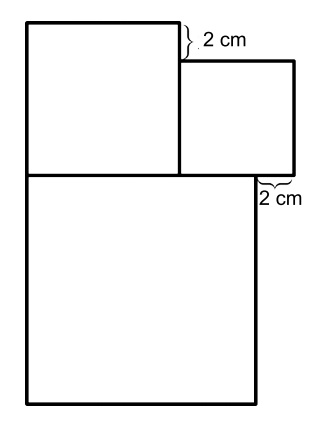
\includegraphics[width=0.4\linewidth]{2020_09_12/imgs/basico_perimetro}
				%\caption{}
				\label{fig:basico_perimetro}
			\end{figure}
			
	\item \textbf{(50 puntos)}. Calcular el resultado de la siguiente suma
	\[
	2\left(1-\frac{1}{2}\right) + 3\left(1-\frac{1}{3}\right) + 4\left(1-\frac{1}{4}\right) + \cdots + 19\left(1-\frac{1}{19}\right) + 20\left(1-\frac{1}{20}\right)
	\]
			
	
	\item \textbf{(50 puntos)}. Oscar escribió en una hoja de papel 5 números enteros positivos y se los mostró a Andrés. Andrés dijo ``La suma de estos 5 números es 23'', y Oscar agregó ``Si! y su producto es 2000. Cuál es el mayor de estos 5 números?''
				

	\item \textbf{(50 puntos)}. Cuántos números de cuatro dígitos mayores que 4000 pueden formarse con los dígitos 2,3,4,5 y 6 si ningún dígito aparece mas de una vez en un número?
			
		
	\item \textbf{(50 puntos)}. Pedro hace la siguiente lista de números
	\[
	1,9,9,7,7,\dots
	\]
	todos los elementos de la lista a partir del quinto elemento son iguales a la cifra de las unidades del producto de los anteriores 4 números de la lista. Por ejemplo el quinto elemento de la lista de Pedro es el 7 porque la cifra de las unidades del producto $1\times 9\times 9\times 7$ es $7$. Pedro continúa así agregando términos a su lista. Cuál es el número que está en la posición $2020$?
\end{enumerate}



%------------------------------------------------------------------------------------------------------------   
%----------------------------------                        AVANZADO                       ---------------------------------- 
%------------------------------------------------------------------------------------------------------------ 

\newpage
\section{Nivel Avanzado}\label{avanzado:2020_12_septiembre}

\begin{center}
	\fbox{\fbox{\parbox{6in}{\centering
				\textbf{Tiempo mínimo: } 2 horas y 30 minutos.\\
				\textbf{Tiempo máximo: } 3 horas y 30 minutos.\\	
				\textbf{Procedimientos: }Cada problema debe estar resuelto por escrito, en forma detallada, todos los pasos seguidos para su resolución deben estar bien explicados. Se le brindarán unas hojas grapadas, en la \textit{parte de enfrente} de cada hoja debe estar la solución de los problemas, la \textit{parte posterior} no se leerá pero las operaciones y cálculos deben hacerlos allí. \\
				\textbf{Puntaje: }Cada problema vale 50 puntos, son 5, para un total de 250 puntos.
	}}}
\end{center}


\begin{enumerate}
	\item \textbf{(50 puntos)}. Hallar todos los valores posibles de $n$ para los cuales se cumple que $n$, $n+2$ y $n+4$ son números primos.
	

	\item \textbf{(50 puntos)}. Considere la función $f(x)$ definida en los enteros positivos. Esta función cumple con la siguiente propiedad:
	\[
	f(xy)=f(x) + f(y)
	\]	
	para cualesquiera enteros positivos $x$ e $y$. Si se sabe que $f(2048)=33$. Calcular el valor de $f(1024)$.
	
	\item \textbf{(50 puntos)}. Cuál es la mayor potencia de $3$ que divide a $25!+26!+27!$?

	\item \textbf{(50 puntos)}. Calcular el área azul en la siguiente figura
	\begin{figure}[H]
		\centering
		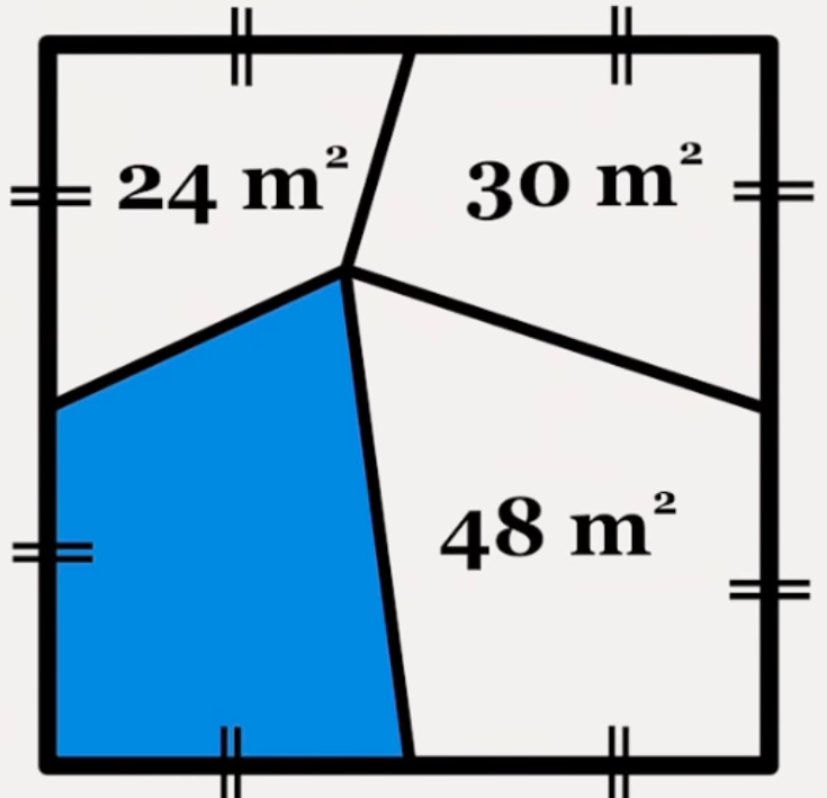
\includegraphics[width=0.4\linewidth]{2020_09_12/imgs/geometria}
		%\caption{}
		\label{fig:geometria}
	\end{figure}


	\item \textbf{(50 puntos)}. Se tiene un cubo. Cuántos planos diferentes existen tales que contengan por lo menos 3 vértices del cubo?

\end{enumerate}
	
	\chapter{10 de Octubre  de 2020}\label{chap:10octubre2020}
	\newpage
\section*{Referencias}
\textbf{Básico: }
\begin{itemize}
	\item \textit{Problema 1.} Creado.
	\item \textit{Problema 2.} \textbf{Creado }.
	\item \textit{Problema 3.} OBMEP 2010, Nivel 1, problema 32.
	\item \textit{Problema 4.} Creado.
	\item \textit{Problema 5.} Problema 6, taller de Áreas de la Universidad de Antioquia.
\end{itemize}

\textbf{Avanzado: }
\begin{itemize}
	\item \textit{Problema 1.} Problema 3 Geometría Nivel 2 Aula 4 , Programa Olimpico Treinamento POTI.
	\item	\textit{Problema 2.} Problem 8, Section ''Integers`` (p. 3) del libro ''Mathematical problems and puzzles`` de S. Straszeuiez. 
	\item	\textit{Problema 3.} Creado.
	\item	\textit{Problema 4.} Problema 10, taller de Polinomios de la Universidad de Antioquia.
	\item	\textit{Problema 5.} Creado.
\end{itemize}

%------------------------------------------------------------------------------------------------------------   
%----------------------------------                        BASICO                       ---------------------------------- 
%------------------------------------------------------------------------------------------------------------ 

\newpage
\section{Nivel Básico}\label{basico:2020_10_octubre}

\begin{center}
	\fbox{\fbox{\parbox{6in}{\centering
				\textbf{Tiempo mínimo: } 2 horas y 30 minutos.\\
				\textbf{Tiempo máximo: } 4 horas.\\	
				\textbf{Procedimientos: }Cada problema debe estar resuelto por escrito, en forma detallada, todos los pasos seguidos para su resolución deben estar bien explicados. Se le brindarán unas hojas grapadas, en la \textit{parte de enfrente} de cada hoja debe estar la solución de los problemas, la \textit{parte posterior} no se leerá pero las operaciones y cálculos deben hacerlos allí. \\
				\textbf{Puntaje: }Cada problema vale 50 puntos, son 5, para un total de 250 puntos.
				}}}
\end{center}

\begin{enumerate}
	\item \textbf{(50 puntos)}.  Cuántos triángulos isósceles diferentes de perímetro 30cm se pueden construir con lados de longitud entera? 
			
	\item \textbf{(50 puntos)}. Un mago le pide a un niño que piense tres números naturales diferentes. El mago es un gran mago y siempre logra adivinar los números que las personas están pensando, pero esta vez se le ha quedado su sombrero en casa y ha perdido toda la magia. Para intentar adivinar los números que el niño está pensando, le pide que le diga cuánto es el producto de ellos, a lo que el niño le responde: 'El producto de los numeros que estoy pensando es  210'. El mago sigue sin adivinar, y el niño le dice otra pista: 'Ninguno de mis números es el 1'. Ayudale al mago diciendole todos los posibles números que puede estar pensando el niño.
			
	
	\item \textbf{(50 puntos)}. Una correa cuadriculada tiene 5 cuadraditos de altura y 250 cuadraditos de ancha como se muestra en la figura \ref{fig:correa_cuadraditos}. Algunos cuadraditos están pintados de gris en sig-sag, comenzando en la izquierda y continuando hacia la derecha con el mismo patrón hasta terminar la correa. Cuántos cuadraditos no están pintados?
				
	\begin{figure}[H]
		\centering
		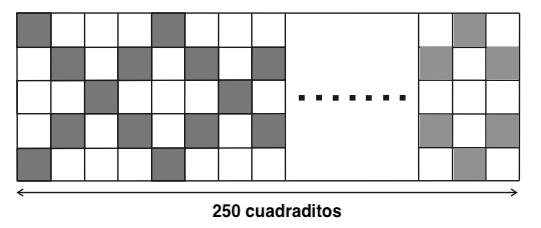
\includegraphics[width=0.8\linewidth]{2020_10_10/imgs/basico_faja_cuadraditos}
		\caption{Correa de cuadraditos.}
		\label{fig:correa_cuadraditos}
	\end{figure}

	\item \textbf{(50 puntos)}. Juan y Sofía están organizando la biblioteca del colegio. La biblioteca solamente tiene 12 libros, todos diferentes. Juan y Sofía los quieren organizar y se dan cuenta que hay 5 en español, 3 en inglés y 4 en francés. Si para organizarlos deciden colocarlos todos sobre un mismo estante,
	\begin{enumerate}[label=\Alph*)]
		\item de cuántas maneras diferentes pueden organizar los libros?
		\item de cuántas maneras diferentes pueden organizar los libros, si los libros que están escritos en el mismo idioma deben quedar juntos?
	\end{enumerate}
		
	\item \textbf{(50 puntos)}. En la figura \ref{fig:area_faja_cuadrado}, el cuadrado $ABCD$ tiene lado de longitud $2cm$. $M$ es punto medio de $BC$ y $N$ es punto medio de $DC$. Calcular el área del cuadrilátero $DNMB$?
	
	\begin{figure}[H]
		\centering
		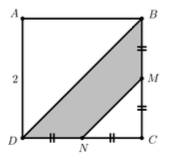
\includegraphics[width=0.5\linewidth]{2020_10_10/imgs/area_faja_cuadrado}
		\caption{Cuadrado $ABCD$ de lado $2cm$. }
		\label{fig:area_faja_cuadrado}
	\end{figure}
	
\end{enumerate}



%------------------------------------------------------------------------------------------------------------   
%----------------------------------                        AVANZADO                       ---------------------------------- 
%------------------------------------------------------------------------------------------------------------ 

\newpage
\section{Nivel Avanzado}\label{avanzado:2020_10_octubre}

\begin{center}
	\fbox{\fbox{\parbox{6in}{\centering
				\textbf{Tiempo mínimo: } 2 horas y 30 minutos.\\
				\textbf{Tiempo máximo: } 4 horas.\\		
				\textbf{Procedimientos: }Cada problema debe estar resuelto por escrito, en forma detallada, todos los pasos seguidos para su resolución deben estar bien explicados. Se le brindarán unas hojas grapadas, en la \textit{parte de enfrente} de cada hoja debe estar la solución de los problemas, la \textit{parte posterior} no se leerá pero las operaciones y cálculos deben hacerlos allí. \\
				\textbf{Puntaje: }Cada problema vale 50 puntos, son 5, para un total de 250 puntos.
	}}}
\end{center}


\begin{enumerate}
	\item \textbf{(50 puntos)}. Sea $ABC$ un triángulo equilatero de lado $20cm$. Una recta pasa por el punto medio $M$ en el lado $AB$ y un punto $N$ en el lado $AC$ y corta a la recta $\overleftrightarrow{BC}$ en el punto $P$ de modo que $CP=12cm$. Hallar la longitud de $NA$.
	

	\item \textbf{(50 puntos)}. Probar que el número $2^{55}+1$ es divisible por 11.
	

	\item \textbf{(50 puntos)}.  Cuántas palabras diferentes se pueden crear con usando exactamente las mismas letras de la palabra \[\textit{''MARAVILLA``}?\] (\textbf{Nota}: ''MARAVILLA`` tiene nueve letras. Una palabra es la union deletras, por ejemplo: ''MARALLAVI``. ).

	\item \textbf{(50 puntos)}. Sean $r_1$ y $r_2$ las raices (soluciones) de la ecuación cuadrática $x^2+px+q=0$. Si se sabe que $r_1 - 2r_2=2$ y $2r_1 -3r_2=5$, encontrar el valor de los coeficientes $p$ y $q$ de la ecuación cuadrática.

	\item \textbf{(50 puntos)}. Sea $ABC$ un triángulo isósceles en $B$, es decir $AB=BC$. Demostrar que la bisectriz, mediana y mediatriz del vértice $B$ son el mismo segmento.

\end{enumerate}
	
	\chapter{31 de Octubre  de 2020}\label{chap:2020_10_31}
	\newpage
\section*{Referencias}
\textbf{Básico: }
\begin{itemize}
	\item \textit{Problema 1.} Creado.
	\item \textit{Problema 2.} Creado. 
	\item \textit{Problema 3.} Creado.
	\item \textit{Problema 4.} Creado.
	\item \textit{Problema 5.} Problema 7, Nivel 1, 3a RONDA ZONAL de OMAPA, 2014.
\end{itemize}

\textbf{Avanzado: }
\begin{itemize}
	\item \textit{Problema 1.} Creado
	\item	\textit{Problema 2.} Problema 24, AMC8, 1997. 
	\item	\textit{Problema 3.} Problema 24, AMC10, 2008. 
	\item	\textit{Problema 4.} Problema 16.11 de Aops Algebra.
	\item	\textit{Problema 5.} Creado.
	\item \textit{Plus} 5.51 de Introduction to Geometry (AOPS).
\end{itemize}

%------------------------------------------------------------------------------------------------------------   
%----------------------------------                        BASICO                       ---------------------------------- 
%------------------------------------------------------------------------------------------------------------ 

\newpage
\section{Nivel Básico}\label{basico:2020_10_31}

\begin{center}
	\fbox{\fbox{\parbox{6in}{\centering
				\textbf{Tiempo mínimo: } 2 horas y 30 minutos.\\
				\textbf{Tiempo máximo: } 4 horas.\\	
				\textbf{Procedimientos: }Cada problema debe estar resuelto por escrito, en forma detallada, todos los pasos seguidos para su resolución deben estar bien explicados. Se le brindarán unas hojas grapadas, en la \textit{parte de enfrente} de cada hoja debe estar la solución de los problemas, la \textit{parte posterior} no se leerá pero las operaciones y cálculos deben hacerlos allí. \\
				\textbf{Puntaje: }Cada problema vale 50 puntos, son 5, para un total de 250 puntos.
				}}}
\end{center}

\begin{enumerate}
	\item \textbf{(50 puntos)}. Mario tiene una bóveda secreta en su habitación, para abrirla debe escribir tres números uno seguido de otro separados por un guión. Un día vió que su hermana estaba intentando adivinar la clave de su bóveda, entonces decidió cambiar su contraseña $12-5-13$ por una nueva. Al día siguiente de cambiar la contraseña intentó abrir la bóveda pero no logró acordarse de su nueva contraseña, solo recuerda que el producto de los números de ella es $210$. Cuántas son las posibles contraseñas que puede tener la bóveda de Mario? (Nota, el orden de introducir los números en la bóveda genera diferentes contraseñas, es decir, la contraseña $2-3-5$ es diferente de la $2-5-3$)
			
	\item \textbf{(50 puntos)}. Cuántos números naturales menores a 1000 dejan residuo 1 al ser divididos por 7? (Recuerde que residuo es el resto que queda al hacer una división, por ejemplo 23 deja residuo 2 al ser dividido por 7)
			
	
	\item \textbf{(50 puntos)}. En un colegio hay 170 estudiantes. Algunos de ellos asisten a la lúdica de Club matemático,  cine o fútbol, que se realizan por las tardes. Se sabe que
			\begin{itemize}
				\item 65 estudiantes asisten a Club matemático.
				\item 96 asisten a cine.
				\item 94 asisten a fútbol.
				\item 35 estudiantes asisten únicamente a la lúdica de cine.
				\item 42 asisten a cine y fútbol.
				\item 40 asisten a Club matemático y fútbol.
				\item 22 estudiantes asisten a las tres lúdicas.
			\end{itemize}
			Con base en la información anterior,
			\begin{enumerate}
				\item ¿Cuántos estudiantes están únicamente en el Club matemático?
				\item ¿Cuántos están únicamente en fútbol?
				\item ¿Cuántos de ellos asisten a cine o fútbol?
				\item ¿Cuántos asisten por lo menos a una de las lúdicas?
				\item ¿Cuántos estudiantes no asisten a ninguna lúdica?
			\end{enumerate}

				

	\item \textbf{(50 puntos)}. María está jugando con su calculadora, sin embargo su calculadora tiene dos problemas, el primero es que solo tiene un botón que lo que hace es multiplicar por 7 el número que esté en la pantalla y el otro problema es que en la pantalla solo muestra la cifra de las unidades del resultado. Por ejemplo, si había un 8 en la pantalla, al oprimir el botón quedará un 6, pues 6 es la cifra de las unidades de $8\times 7 =56$. Si al inicio María ve el número 7 en la pantalla, que número quedará en la pantalla luego de que María oprima el botón 2020 veces?
			
		
	\item \textbf{(50 puntos)}. Las cuadrículas del gráfico \ref{fig:omapa} son todas iguales. El área pintada de negro es de $72{\text{ cm}}^2$. Cuánto es la suma de las áreas de los triángulos $ABC$ y $CDE$?
	\begin{figure}[H]
		\centering
		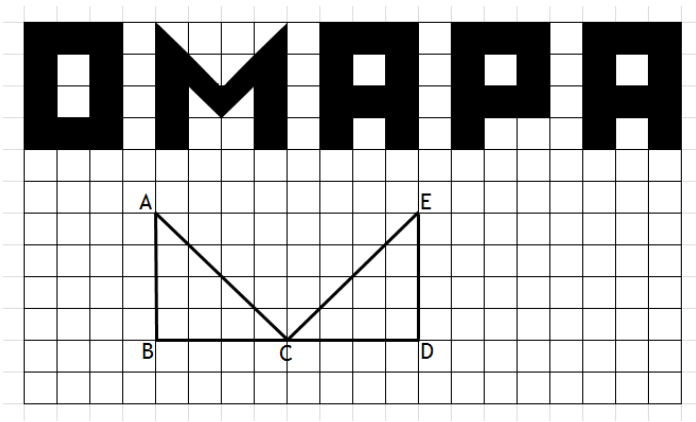
\includegraphics[width=0.7\linewidth]{2020_10_31/imgs/omapa}
		%\caption{}
		\label{fig:omapa}
	\end{figure}
	
\end{enumerate}



%------------------------------------------------------------------------------------------------------------   
%----------------------------------                        AVANZADO                       ---------------------------------- 
%------------------------------------------------------------------------------------------------------------ 

\newpage
\section{Nivel Avanzado}\label{avanzado:2020_10_31}

\begin{center}
	\fbox{\fbox{\parbox{6in}{\centering
				\textbf{Tiempo mínimo: } 2 horas y 30 minutos.\\
				\textbf{Tiempo máximo: } 4 horas.\\		
				\textbf{Procedimientos: }Cada problema debe estar resuelto por escrito, en forma detallada, todos los pasos seguidos para su resolución deben estar bien explicados. Se le brindarán unas hojas grapadas, en la \textit{parte de enfrente} de cada hoja debe estar la solución de los problemas, la \textit{parte posterior} no se leerá pero las operaciones y cálculos deben hacerlos allí. \\
				\textbf{Puntaje: }Cada problema vale 50 puntos, son 5, para un total de 250 puntos.
	}}}
\end{center}


\begin{enumerate}
	\item \textbf{(50 puntos)}. Cuántos números entre $-1000$ y $1000$ dejan residuo 5 al dividirlos por 9? (Recuerde que residuo es el resto que queda al hacer una división, por ejemplo -7 deja residuo 3 al ser dividido por 5, porque $-7=\color{red}5\color{black} \times (-2) + 3$. )
	

	\item \textbf{(50 puntos)}. En la figura \ref{fig:AV1} los vértices $A,C$ y $E$ están sobre el diámetro del circulo y el vértice $C$ divide al segmento $AE$ a razón de $2:3$. Los dos semicírculos, $ ABC $ y $ CDE $, dividen al circulo en una región superior (sombreada) y una región inferior. Cuál es la razón entre el área de la región superior y la de la región inferior.	
		\begin{figure}[H]
			\centering
			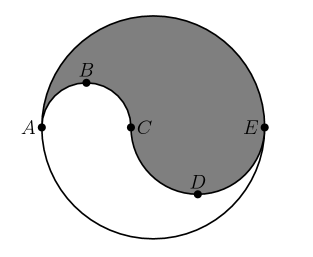
\includegraphics[width=0.5\linewidth]{2020_10_31/imgs/AV1}
			%\caption{}
			\label{fig:AV1}
		\end{figure}
	
	\item \textbf{(50 puntos)}.  Sea $ k = 2008 ^ 2 + 2 ^ {2008} $. ¿Cuál es el dígito de las unidades de $ k ^ 2 + 2 ^ k $?

	\item Sea $f(x)$ la función $f(x) = 3x+10$.
	\begin{enumerate}
		\item \textbf{(5 puntos)}. Calcular $f(2)$.		
		\item \textbf{(10 puntos)}. Calcular $f(f(3))$.
		\item \textbf{(35 puntos)}. Para que valores de $x$ se cumple que $f(f(x))=x?$
	\end{enumerate} 

	\item \textbf{(50 puntos)}. En total, en el club matemático de bachillerato hay 7 mujeres y 5 hombres. Necesito elegir un equipo con 5 personas para que participe de una prueba por equipos. De cuántas maneras diferentes puedo seleccionar el equipo
		\begin{enumerate}
			\item \textbf{(10 puntos)}. si no hay ninguna restricción para elegir los participantes del equipo? 
			\item \textbf{(15 puntos)}. si tienen que haber 2 mujeres y 3 hombres en el equipo? 
			\item \textbf{(25 puntos)}. si tienen que haber mas mujeres que hombres en el equipo? 
		\end{enumerate} 
	
	\item \textbf{PLUS (50 puntos)}. En la figura \ref{challege_551_aopgeo_ejer},  $\overline{BC} \parallel \overline{UR}$, $\overline{PS} \parallel \overline{BA}$ y $\overline{TQ} \parallel \overline{AC}$. Probar que
	\[
	\frac{PQ}{BC} + \frac{RS}{CA} + \frac{TU}{AB} = 1
	\]
	\begin{figure}[H]
		\centering
		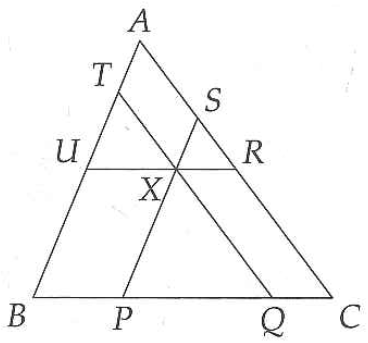
\includegraphics[width=0.5\linewidth]{2020_10_31/imgs/challege_551_aopgeo_ejer}		
	\end{figure}

\end{enumerate}
	
	\chapter{15 de marzo de 2021}
	\newpage
\section*{Referencias}
\textbf{Básico: }
\begin{itemize}
	\item \textit{Problema 1.} Creado 
	\item \textit{Problema 2.} UAN Clasificatorio Basico 2017.
	\item \textit{Problema 3.} UAN Clasificatorio Basico 2017.
	\item \textit{Problema 4.} UAN Clasificatorio Basico 2017.
\end{itemize}

\textbf{Avanzado: }
\begin{itemize}
	\item \textit{Problema 1.} 
	\item	\textit{Problema 2.} 
	\item	\textit{Problema 3.} 
	\item	\textit{Problema 4.}
	\item	\textit{Problema 5.} 
\end{itemize}

%------------------------------------------------------------------------------------------------------------   
%----------------------------------                        BASICO                       ---------------------------------- 
%------------------------------------------------------------------------------------------------------------ 

\newpage
\section{Nivel Básico}

\begin{center}
	\fbox{\fbox{\parbox{6in}{\centering
				\textbf{Tiempo: } 2 horas.\\
				\textbf{Procedimientos: }Cada problema debe estar resuelto por escrito en papel, en forma detallada, todos los pasos seguidos para su resolución deben estar bien explicados. Se le brindarán unas hojas grapadas, en la \textit{parte de enfrente} de cada hoja debe estar la solución de los problemas, la \textit{parte posterior} no se leerá pero las operaciones y cálculos deben hacerlos allí. \\
				\textbf{Puntaje Máximo: } 300 puntos.
				}}}
\end{center}

\begin{enumerate}
	\item \textbf{(100 puntos)}. Para año nuevo Mario se promete ahorrar en su alcancia 5 monedas el día primer día del año, 10 monedas el día segundo del año, 15 monedas el tercer día, 20 el cuarto día y así sucesivamente.
	\begin{enumerate}[label=\Alph*)]
		\item Cuántos días hay desde el primer día (contandolo) en el que mete 5 monedas hasta el día en que mete 200 monedas en la alcancía?
		
		\item Cuántas monedas habrá en su alcancia luego de que meta las 200 monedas ese día? 
		
		\item Si ahorra con monedas de 50 pesos, cuanto ahorrará en 365 dias?
		
		\item Mario quiere comprar una casa que cuesta $100.000.000$. Si continúa ahorrando de esta manera, cuántos días tienen que pasar para poder comprarla?
	\end{enumerate}
			

	\item \textbf{(50 puntos)}. Encontrar el valor de la expresión:
	\[100-98+96-94+92-90+\cdots +8-6+4-2\]
	
				
	\item \textbf{(30 puntos)}.  ¿Cuál es la suma de los diferentes divisores enteros primos de
	2016?
			
		
	\item \textbf{(60 puntos)}. Una contraseña de una tarjeta débito en el banco de Federico
	está compuesta por cuatro cifras de 0 a 9 que se pueden repetir.	Si ninguna contraseña puede comenzar con la secuencia 9, 1, 1,
	¿Cuántas contraseñas se pueden generar?
	
	\item \textbf{(60 puntos)}. La suma de 25 enteros pares consecutivos es 10, 000. ¿Cuál es
	el mayor de estos 25 enteros pares consecutivos?
	
\end{enumerate}



%------------------------------------------------------------------------------------------------------------   
%----------------------------------                        AVANZADO                       ---------------------------------- 
%------------------------------------------------------------------------------------------------------------ 

\newpage
\section{Nivel Avanzado}

\begin{center}
	\fbox{\fbox{\parbox{6in}{\centering
				\textbf{Tiempo mínimo: } 2 horas y 30 minutos.\\
				\textbf{Tiempo máximo: } 4 horas.\\		
				\textbf{Procedimientos: }Cada problema debe estar resuelto por escrito, en forma detallada, todos los pasos seguidos para su resolución deben estar bien explicados. Se le brindarán unas hojas grapadas, en la \textit{parte de enfrente} de cada hoja debe estar la solución de los problemas, la \textit{parte posterior} no se leerá pero las operaciones y cálculos deben hacerlos allí. \\
				\textbf{Puntaje: }Cada problema vale 50 puntos, son 5, para un total de 250 puntos.
	}}}
\end{center}


\begin{enumerate}
	\item \textbf{(50 puntos)}. 
	

	\item \textbf{(50 puntos)}. 
	

	\item \textbf{(50 puntos)}.  

	\item \textbf{(50 puntos)}. 

	\item \textbf{(50 puntos)}. 

\end{enumerate}
		
		
\end{document}